\documentclass[12pt]{article}
\usepackage[english]{babel}
\usepackage{amsmath,amsthm,amsfonts,amssymb,epsfig, graphicx, listings}
\usepackage[left=1in,top=1in,right=1in]{geometry}
\title{Varying Coefficient Model}
\author{David Flatow}
\date{}

\newcommand{\E}{\mathbb{E}}
\newcommand{\I}{\mathbb{I}}
\newcommand{\bhat}{\hat{\beta}}
\newcommand{\tB}{\tilde{\beta}}
\newcommand{\B}{\beta}
\newcommand{\tX}{\tilde{X}}
\newcommand{\R}{\mathbb{R}}
\newcommand{\Det}{\textbf{det}}
\newcommand{\benum}{\begin{enumerate}}
\newcommand{\enum}{\end{enumerate}}
\newcommand{\bmat}{\begin{bmatrix}}
\newcommand{\emat}{\end{bmatrix}}
\newcommand{\one}{\textbf{1}}
\newcommand{\zero}{\textbf{0}}
\newcommand{\order}{\mathcal{O}}
\newcommand{\br}{\bigg]}
\newcommand{\bl}{\bigg[}
\newcommand{\pr}{\bigg)}
\newcommand{\pl}{\bigg(}
\newcommand{\eps}{\varepsilon}


\newcommand{\e}{\varepsilon}
\newcommand{\bb}{\mathbb}
\newcommand{\var}{\text{Var}}
\newcommand{\cov}{\text{Cov}}
\newcommand{\bcase}{\begin{cases}}
\newcommand{\ecase}{\end{cases}}
\newcommand{\blist}{\begin{enumerate}}
\newcommand{\elist}{\end{enumerate}}
\newcommand{\bproof}{\begin{proof}}
\newcommand{\eproof}{\end{proof}}
\newcommand{\bsol}{\bproof[Solution]}
\newcommand{\esol}{\eproof}
\newcommand{\til}{\tilde}
\newcommand{\bbar}{\overline}
\newcommand{\grad}{\nabla}
\newcommand{\argmax}{\text{argmax}}
\newtheorem{thm}{Theorem}[section]
\newtheorem{lem}[thm]{Lemma}
\newtheorem{prop}[thm]{Proposition}
\newtheorem{cor}[thm]{Corollary}
\newtheorem{df}[thm]{Definition}


\usepackage{color}

\definecolor{dkgreen}{rgb}{0,0.6,0}
\definecolor{gray}{rgb}{0.5,0.5,0.5}
\definecolor{mauve}{rgb}{0.58,0,0.82}

\lstset{frame=tb,
  language=R,
  aboveskip=3mm,
  belowskip=3mm,
  showstringspaces=false,
  columns=flexible,
  basicstyle={\small\ttfamily},
  numbers=none,
  numberstyle=\tiny\color{gray},
  keywordstyle=\color{blue},
  commentstyle=\color{dkgreen},
  stringstyle=\color{mauve},
  breaklines=true,
  breakatwhitespace=true, 
  tabsize=3
}

\begin{document}

\maketitle

\blist

\item You have a set of $p$ variables in the matrix $X$ which represent some economic indicators measured over a number of years, and a response $y$ also measured for the same years. You fit a linear model, but are criticized because you are told that the regime changes in time, and so should your model. You decide to let your regression coefficients (and intercept) change smoothly with time, a so-called varying coefficient model.

\blist

\item Since we want $\B_i$ to be a smooth function of time we express it in the basis space of a natural cubic spline of $t$:
$$ \B_i(t) = \sum_{j=1}^m h_j(t)\theta_{ij} = h(t)^T\theta_{i}$$
Then our time series model is,
$$y(t) = \B_0(t) + \B_1(t)x_1(t) + \B_2(t)x_2(t)$$
$$ = h(t)^T\theta_0 + x_1(t)h(t)^T\theta_1 +  x_2(t)h(t)^T\theta_2 $$
$$ = H(t)\theta $$
Where $H(t) = \bmat - h(t)^T - & - x_1(t)h(t)^T-& -x_2(t)h(t)^T - \emat $. And so,
$$ H = \bmat | & | & |  \\ - h^T - & - x_1h^T - & - x_2h^T - \\ | & | & | \emat $$
But this is a linear model in the design matrix $H$. And so we have,
$$ y = H\theta $$
And we can estimate $\theta$ by OLS. Once we have our estimates $\hat{\theta}$ we can back out our time varying estimates for $\hat{\B}_j(t)$. Specifically, 

$$ \hat{\B_j} = h^T\hat{\theta_j}$$


\item We read in the data in vcdata.csv. There is a two-column $x$ and a time variable $t$. We fit the varying coefficient model, and plot the three coefficient functions versus time. We compute the point-wise standard errors for each of these, and include a standard-error band (upper and lower) for each function.

We can compute the variance-covariance matrix of $\hat{\B_j}$ as follows:

$$\Sigma_j = Var(\hat{\B_j}) = Var(h^T\hat{\theta_j}) = h^T Var(\hat{\theta_j})h$$

Note that $Var(\hat{\theta_j})$ is sub-block of the usual variance-covariance matrix of $\hat{\theta}$ in the OLS estimation of $\hat{\theta}$ in the model $y = H\theta$. Specifically, it is the block $\Sigma_{\theta}[j:j+df, j:j+df]$. Then the point-wise standard errors of $\hat{\beta_j}$ are given by the square root of the diagonal of $\Sigma_j$ and confidence bands are given by $\beta_j \pm 2 \sqrt{diag(\Sigma_j)}$.

We can implement this in $R$ as follows:

\lstinputlisting{./code/VCM.R}

\begin{center}
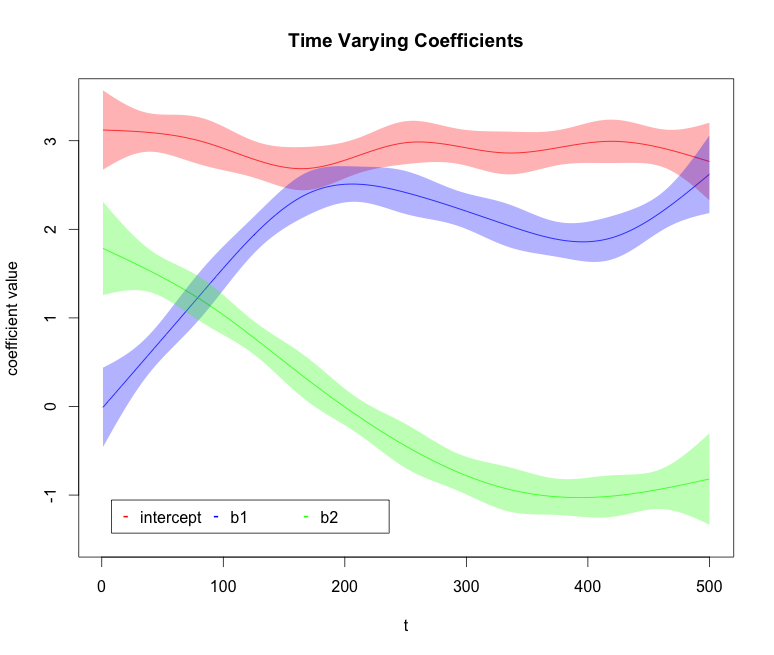
\includegraphics[width=0.8\textwidth]{./figures/4.png}
\end{center}



\elist
\elist

\end{document}